% file: graph-paths/dijkstra-correctness.tex

\documentclass[tikz]{standalone}

\usetikzlibrary{positioning, shapes, arrows.meta, decorations.pathmorphing, backgrounds, fit}

\begin{document}
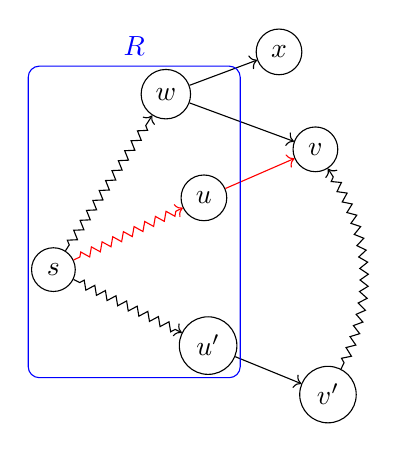
\begin{tikzpicture}[n/.style = {circle, draw}, % node
    leadsto/.style = {->, decorate, decoration = {
    	zigzag, amplitude = 1.50pt, segment length = 1.5mm, pre length = 2.5pt, post length = 2.5pt}},
    e/.style = {->}, % edge
  ]
  \node (s) [n] {$s$};

  \node (u) [n, above right = 0.5cm and 1.50cm of s] {$u$};
  \node (u') [n, below right = 0.5cm and 1.50cm of s] {$u'$};
  \node (w) [n, above right = 1.8cm and 1.00cm of s] {$w$};

  \node (v) [n, above right = 0.2cm and 1.00cm of u] {$v$};
  \node (v') [n, below right = 0.1cm and 1.00cm of u'] {$v'$};
  \node (x) [n, above right = 0.1cm and 1.00cm of w] {$x$};

  \path (s) edge[leadsto, red] (u)
	    edge[leadsto] (u')
	    edge[leadsto] (w)
	(u) edge[e, red] (v)
	(u') edge[e] (v')
	(w) edge[e] (x)
	    edge[e] (v)
	(v') edge[leadsto, bend right] (v);

  \node[draw, blue, fit = (s) (w) (u) (u'), rectangle, rounded corners, inner sep = 1pt, label = {[blue] above: $R$}] {};
\end{tikzpicture}
\end{document}